\documentclass{article}
\usepackage{amsthm}
\usepackage{amsmath}
\usepackage{float}
\usepackage[dvipsnames]{xcolor}
\usepackage{colortbl}
\usepackage{avant}
\usepackage{fancyhdr}
\usepackage{tikz}
\usetikzlibrary{shapes}
\usepackage{hyperref}
\usepackage[bottom]{footmisc}
\usepackage{caption}

\captionsetup[table]{labelformat=empty}

\renewcommand{\familydefault}{\sfdefault}   % cambio font
\theoremstyle{definition}
\newtheorem*{definition}{Definizione}
\renewcommand{\figurename}{Figura}
\renewcommand{\contentsname}{Contenuti}

\pagestyle{fancy}
\fancyfoot[L]{Basi di Dati}
\fancyfoot[C]{\thepage}
\fancyfoot[R]{Angelo Passarelli}

\setcounter{section}{-1}

\title{Basi di Dati}
\author{Angelo Passarelli}
\date{\today}

\begin{document}    
    \maketitle
    \begin{center}
        
\includegraphics[scale=0.15]{img/Stemma_unipi.png}
    \end{center}
    \vspace{1cm}
    \begin{center}
        Appunti basati sulle lezioni e dispense della professoressa Giovanna Rosone \footnote{\url{https://pages.di.unipi.it/rosone/index.html}}
    \end{center}
    \pagebreak
    \tableofcontents
    \pagebreak

    \begin{sloppypar}

    \section{Introduzione}

    \begin{definition}[Base di Dati]
        Una base di dati è un insieme organizzato di dati utilizzati per il supporto allo svolgimento di attività.
    \end{definition}

    \paragraph*{Struttura dei Dati}
    I dati sono organizzati in insiemi strutturati che possono presentare fra loro delle relazioni. Tuple che rappresentano dati nello stesso insieme devono essere omogenee ed univoche.

    \begin{definition}[Sistema Informativo]
        Un sistema informativo è una combinazione di risorse umane e/o materiali e procedure organizzate per
        la \textcolor{purple}{raccolta}, l'\textcolor{purple}{archiviazione}, l'\textcolor{purple}{elaborazione}
        e lo \textcolor{purple}{scambio} di informazioni necessarie ad un'attività, le quali possono essere classificate in:
        \begin{itemize}
            \item Informazioni di servizio (operative).
            \item Informazioni di controllo (pianificazione e gestione).
            \item Informazioni di governo (pianificazione strategica).
        \end{itemize}
        \begin{figure}[h]
            \centering
            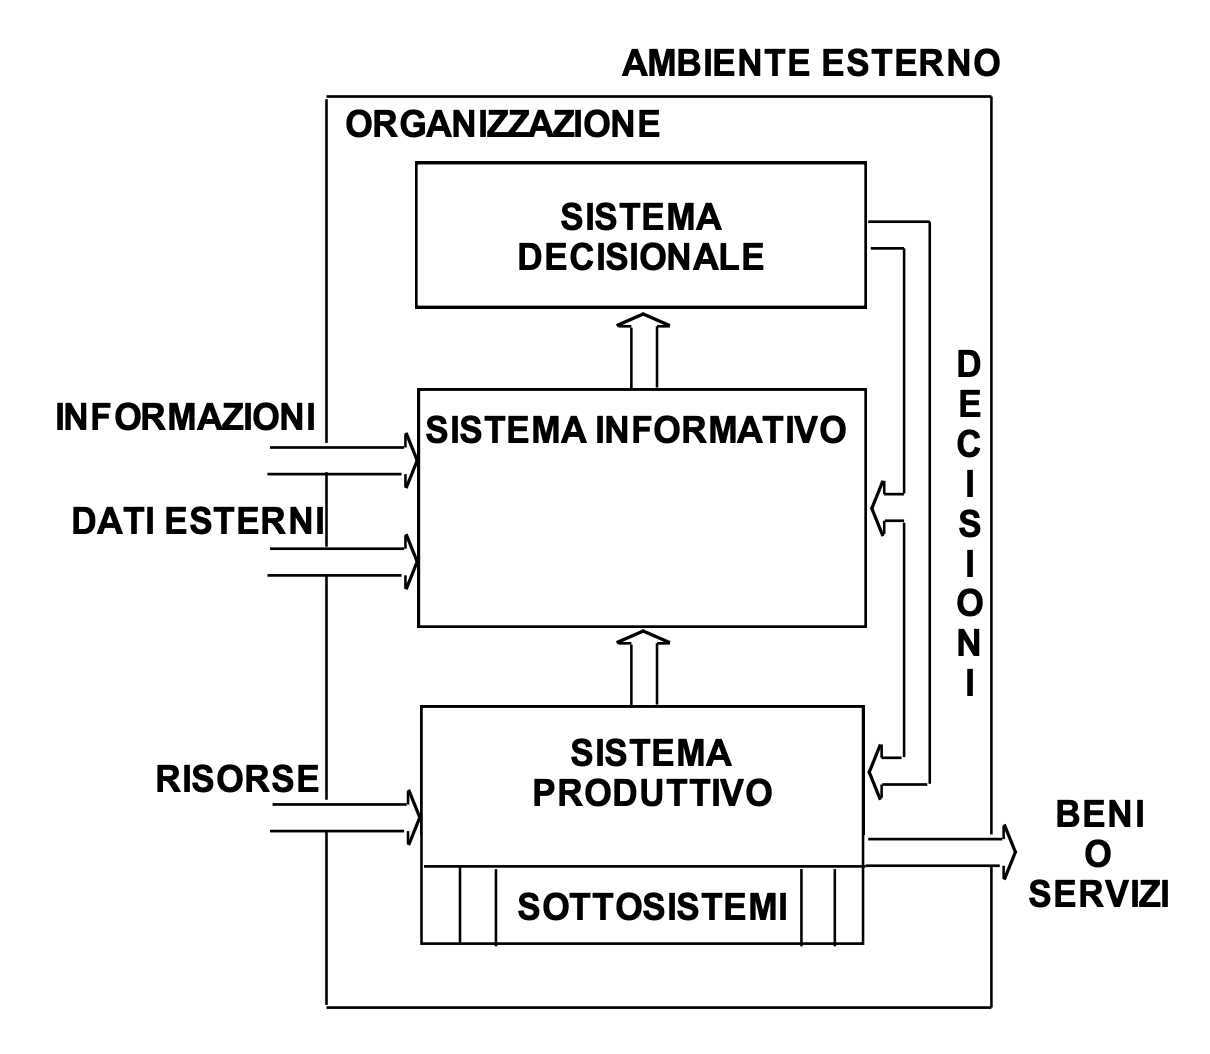
\includegraphics[scale=0.5]{img/sistema_informativo.png}
            \caption{Esempio di sistema informativo}
        \end{figure}
    \end{definition}

    \begin{definition}[Sistema Informativo Automatizzato]
        Un sistema informativo automatizzato è una parte del sistema informativo che permette di implementare le procedure
        che si occupano della gestione delle informazioni usando un sistema informatico.
    \end{definition}

    \begin{definition}[Sistema Informatico]
        Un sistema informatico è l'insieme delle tecnologie a supporto per le attività di un'organizzazione.
        Si possono classificare in:
        \begin{itemize}
            \item \textbf{\textcolor{purple}{Sistemi informatici operativi}}: questi sistemi si utilizzano per svolgere le normali attività dell'azienda
                per la fruizione del suo bene o servizio, e per la gestione interna dei singoli reparti dell'azienda.
                Le operazioni sui dati in questo sistema sono di tipo \textcolor{purple}{OLTP} (\emph{On-Line Transaction Processing})
                e prevedono elaborazioni semplici che coinvolgono pochi dati che vengono aggiornati molto frequentemente.
            \item \textbf{\textcolor{purple}{Sistemi informatici direzionali}}: i dati sono organizzati in \emph{Data Warehouse}
                che consentono di aiutare l'azienda nei processi di controllo delle prestazioni e di decisione manageriale.
                Le elaborazioni su questo tipo di sistema si chiamano \textcolor{purple}{OLAP} (\emph{On-Line Analytical Processing})
                e prevedono l'utilizzo di una grande mole di dati che sono per lo più storici. In questo caso i dati vengono aggiornati
                molto raramente, ma su di essi vengono svolte molte operazioni, anche da un punto di vista multidimensionale, ovvero
                vengono incrociati più dati per analizzare le informazioni ottenute sotto molteplici punti di vista.
        \end{itemize}
    \end{definition}

    \begin{definition}[DBMS]
        Un \emph{Database Management System} è un sistema che garantisce
        il controllo e la gestione di dati per renderli accessibili agli utenti opportuni in base ai loro privilegi.
        Il DBMS fornisce anche dei linguaggi che permettono di definire lo \textcolor{purple}{schema} di un database, di scegliere le \textcolor{purple}{strutture dati}
        opportune per la memorizzazione dei dati, di rispettare i \textcolor{purple}{vincoli} per ogni tipo di dato e di poter \textcolor{purple}{modificare} e
        \textcolor{purple}{interrogare} il database.
    \end{definition}

    \paragraph*{Metadati} All'interno del database sono anche memorizzati dei metadati che si riferiscono agli utenti
    e allo schema utilizzato dal database stesso. Anche i metadati possono essere interrogati e modificati.
    \section{DBMS e Linguaggi}
Si distinguono tre diversi livelli di descrizione dei dati:
\begin{itemize}
    \item A livello di \textcolor{purple}{\emph{vista} logica}: descrive come deve apparire il database a seconda dell'utente che lo usa, in base ai suoi permessi.
    \item A livello \textcolor{purple}{logico}: descrive la struttura degli insiemi dei dati e le relazioni fra essi,
        senza doversi occupare della loro organizzazione nella memoria.
    \item A livello \textcolor{purple}{fisico}: viene descritto come sono organizzati fisicamente i dati nella memoria e
        vengono riportate quali strutture dati ausiliare vengono utilizzate.
\end{itemize}

\begin{center}
    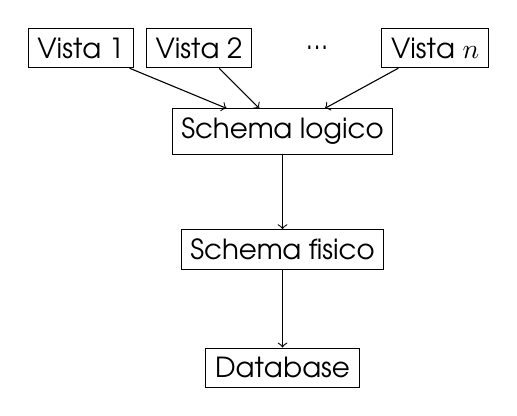
\begin{tikzpicture}[node distance = 1.5cm, main/.style={rectangle, draw}]
        \node[main] (1) {Vista 1};
        \node[main] (2) [right of=1] {Vista 2};
        \node[main, draw opacity=0] (3) [right of=2] {...};
        \node[main] (4) [right of=3] {Vista $n$};
        \node[main] (5) [below right of=2] {Schema logico};
        \node[main] (6) [below of=5] {Schema fisico};
        \node[main] (7) [below of=6] {Database};
        \draw[->] (1) -- (5);
        \draw[->] (2) -- (5);
        \draw[->] (4) -- (5);
        \draw[->] (5) -- (6);
        \draw[->] (6) -- (7);
    \end{tikzpicture}
\end{center}

Quest approccio permette di garantire le proprietà di indipendenza logica e fisica:
\begin{itemize}
    \item \textbf{\textcolor{purple}{Indipendenza Logica}}: gli applicativi non necessitano modifiche in seguite a variazioni dello schema logico.
    \item \textbf{\textcolor{purple}{Indipendenza Fisica}}: gli applicativi non necessitano modifiche in seguito a cambiamenti dell'organizzazione fisica dei dati.
\end{itemize}

Per quanto riguarda i linguaggi di interrogazione, questi possono essere distinti in:
\begin{itemize}
    \item \textbf{\textcolor{purple}{DML}} (Data Manipulation Language): per l'interrogazione e l'aggiornamento dei dati.
    \item \textbf{\textcolor{purple}{DDL}} (Data Definition Language): per la definizione di schemi, sia logici che fisici, ed altre operazioni. 
\end{itemize}

\subsection{Funzionalità del DBMS}
Un DBMS deve prevedere più modalità d'uso per soddisfare le esigenze di più categorie di utenti
che accedono al database. Deve poter offrire:

\begin{itemize}
    \item Un'interfaccia grafica per accedere ai dati.
    \item Un linguaggio di interrogazione per gli utenti inesperti (non programmatori).
    \item Un linguaggio di programmazione per chi sviluppa applicazioni, nello specifico deve prevedere
        l'integrazione del \emph{DDL} e del \emph{DML} nel linguaggio ospite.
    \item Un linguaggio per lo sviluppo di interfacce per le applicazioni.
    \item Predisporre per l'\textcolor{purple}{amministratore} strumenti per stabilire i diritti d'accesso ai dati,
        per il ripristino del sistema e per la modifica e la definizione degli schemi logici (sia interno che esterno).
    
\end{itemize}

\subsection{Proprietà dei Database}
Il DBMS permette di garantire al database le seguenti proprietà:
\begin{itemize}
    \item \textcolor{purple}{Integrità}: mantenimento dei vincoli d'integrità dichiarati in fase di definizione dello schema.
    \item \textcolor{purple}{Affidabilità}: protezione dei dati da parte di malfunzionamenti sia software che hardware e da anomalie indesiderate
        come l'accesso concorrente al database da parte di più utenti.
    \item \textcolor{purple}{Sicurezza}: protezione dei dati da parte di utenti non autorizzati.
\end{itemize}

Inoltre un DBMS deve essere in grado di gestire collezioni di dati che siano:
\begin{itemize}
    \item \textcolor{purple}{Grandi}
    \item \textcolor{purple}{Persistenti}: il periodo di vita dei dati è indipendente dai programmi che li utilizzano.
    \item \textcolor{purple}{Condivise}: possono essere usati da programmi diversi.
\end{itemize}

Il DMBS deve essere anche \textcolor{purple}{efficiente} (utilizzando al meglio le risorse in termini di \emph{spazio} e \emph{tempo}) ed \textcolor{purple}{efficace}.

\subsection{Transazioni}

\begin{definition}[Transazione]
    Una transazione è una serie di azioni di lettura e scrittura sulla memoria permanente
    o di elaborazione dati in memoria temporanea. Presenta le seguenti proprietà:
    \begin{itemize}
        \item \textbf{\textcolor{purple}{Atomicità}}: le transizioni che non vanno a buon fine o che vengono abortite
            sono trattate come se non fossero mai state eseguite.
        \item \textbf{\textcolor{purple}{Persistenza}}: le modifiche effettuate da una transizione andata a buon fine sono permanenti,
            ovvero non possono essere alterate da malfunzionamenti.
        \item \textbf{\textcolor{purple}{Serializzabilità}}: nel caso di esecuzioni concorrenti di più transazioni, l'effetto ottenuto è quello di un'esecuzione seriale.
    \end{itemize}
\end{definition}

\section{Modellazione}
\begin{definition}[Modello Astratto]
    Un modello astratto è la rappresentazione formale di idee e conoscenze relative ad un fenomeno.
\end{definition}

La modellazione è centrale nella progettazione del database che comprende le fasi presenti in figura.
\begin{center}
    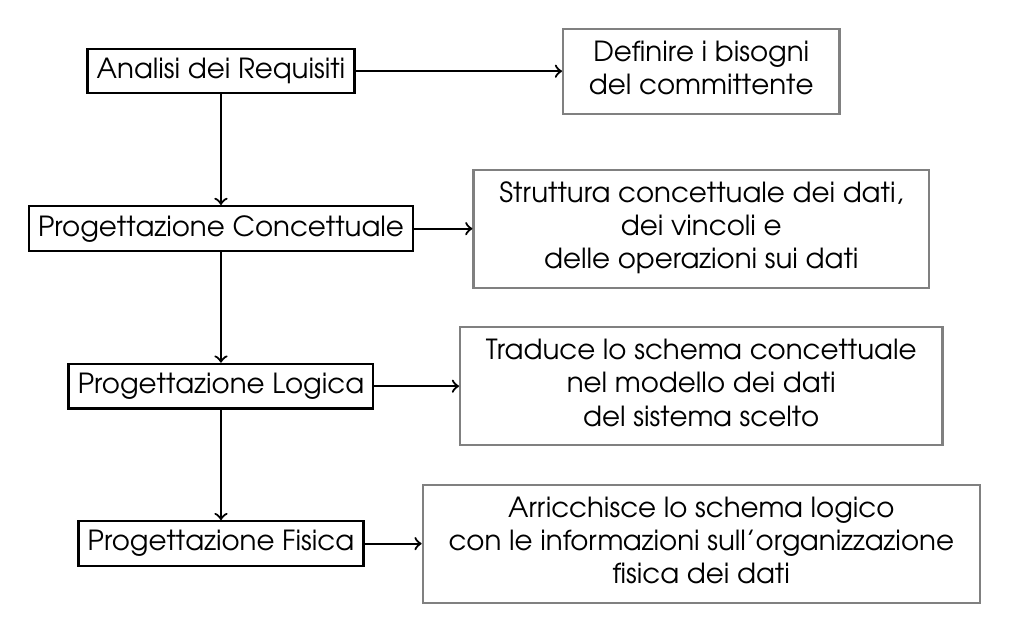
\begin{tikzpicture}[thick, main/.style = {draw, rectangle}, desc/.style = {draw=gray, rectangle}]
        \node[main] (1)  {Analisi dei Requisiti};
        \node[main] (2) [below of=1, node distance = 2cm] {Progettazione Concettuale};
        \node[main] (3) [below of=2, node distance = 2cm] {Progettazione Logica}; 
        \node[main] (4) [below of=3, node distance = 2cm] {Progettazione Fisica};
        \node[desc] (5) [right of=1, node distance = 6.1cm] {\begin{tabular}{c} Definire i bisogni \\ del committente \end{tabular}};
        \node[desc] (6) [below of=5, node distance = 2cm] {\begin{tabular}{c} Struttura concettuale dei dati, \\ dei vincoli e \\ delle operazioni sui dati \end{tabular}};
        \node[desc] (7) [below of=6, node distance = 2cm] {\begin{tabular}{c} Traduce lo schema concettuale \\ nel modello dei dati \\ del sistema scelto \end{tabular}};
        \node[desc] (8) [below of=7, node distance = 2cm] {\begin{tabular}{c} Arricchisce lo schema logico \\ con le informazioni sull'organizzazione \\ fisica dei dati \end{tabular}};
        \draw[->] (1) -- (2);
        \draw[->] (2) -- (3);
        \draw[->] (3) -- (4);
        \draw[->] (1) -- (5);
        \draw[->] (2) -- (6);
        \draw[->] (3) -- (7);
        \draw[->] (4) -- (8);
    \end{tikzpicture}
\end{center}

\subsection{Fasi della Modellazione}

\begin{center}
    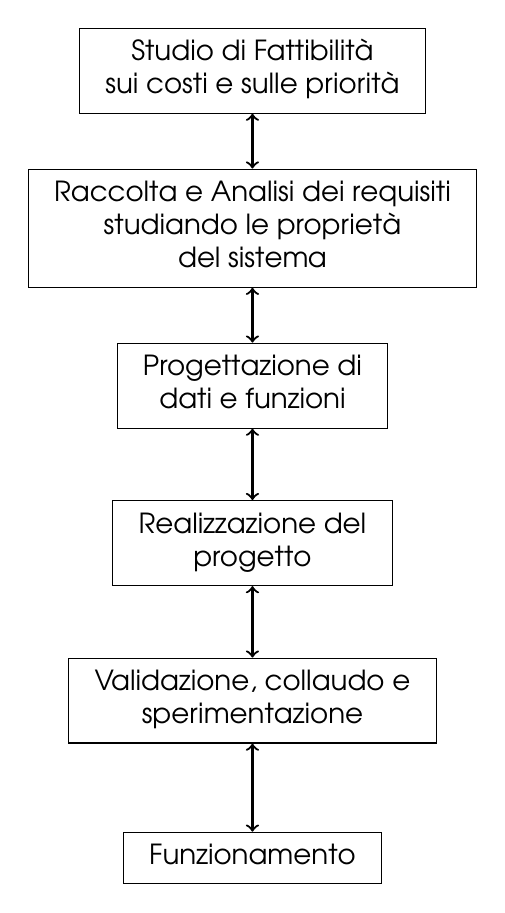
\begin{tikzpicture}[node distance=2cm, main/.style={draw, rectangle}]
        \node[main] (1) {\begin{tabular}{c}Studio di Fattibilità \\ sui costi e sulle priorità\end{tabular}};
        \node[main] (2) [below of=1] {\begin{tabular}{c}Raccolta e Analisi dei requisiti \\ studiando le proprietà \\ del sistema\end{tabular}};
        \node[main] (3) [below of=2] {\begin{tabular}{c}Progettazione di \\ dati e funzioni\end{tabular}};
        \node[main] (4) [below of=3] {\begin{tabular}{c}Realizzazione del \\ progetto\end{tabular}};
        \node[main] (5) [below of=4] {\begin{tabular}{c}Validazione, collaudo e \\ sperimentazione\end{tabular}};
        \node[main] (6) [below of=5] {\begin{tabular}{c}Funzionamento\end{tabular}};
        \draw[<->, thick] (1) -- (2);
        \draw[<->, thick] (2) -- (3);
        \draw[<->, thick] (3) -- (4);
        \draw[<->, thick] (4) -- (5);
        \draw[<->, thick] (5) -- (6);
    \end{tikzpicture}   
\end{center}

\subsection{Analizzare il Dominio}
Il dominio può presentare più aspetti da dover analizzare:
\begin{itemize}
    \item Aspetto \emph{\textcolor{purple}{ontologico}}: conoscere ciò che si suppone esista nell'universo del contesto e quindi ciò che è da modellare.
        Occorre analizzare tre tipi di conoscenze:
        \begin{itemize}
            \item Conoscenza \emph{\textcolor{purple}{concreta}}: le entità del contesto e le associazioni fra di esse.
                \begin{definition}[Entità]
                    Sono oggetti di cui occorre definire le proprietà.
                \end{definition}
                \begin{definition}[Proprietà]
                    Descrivono le caratteristiche di determinate entità e sono formata da una coppia \verb+(Attributo, Valore)+.
                    Ogni proprietà ha ad essa associato un dominio, quindi un insieme di valori che può assumere. Inoltre le proprietà si possono classificare in:
                    \begin{itemize}
                        \item \textcolor{purple}{Atomiche} o \textcolor{purple}{Strutturate}: atomiche se il loro valore non è ulteriormente scomponibile.
                        \item \textcolor{purple}{Totali} o \textcolor{purple}{Parziali}: se è obbligatoria oppure opzionale.
                        \item \textcolor{purple}{Univoche} o \textcolor{purple}{Multivalore}: univoca se per ogni entità la scelta del valore è unico (\emph{es. codice fiscale}).
                        \item \textcolor{purple}{Costanti} o \textcolor{purple}{Variabili}
                        \item \textcolor{purple}{Calcolate} o \textcolor{purple}{Non Calcolate}: calcolata se è possibile derivarla da altre proprietà.
                    \end{itemize}
                \end{definition}
                \begin{definition}[Tipo di un'entità]
                    Ogni entità appartiene ad un tipo che ne indica la propria natura.
                \end{definition}
                \begin{definition}[Collezione]
                    Insieme di entità dello stesso tipo.
                \end{definition}
            \item Conoscenza \emph{\textcolor{purple}{astratta}}: la struttura e i vincoli sulle entità.
            \item Conoscenza \emph{\textcolor{purple}{procedurale}}: le operazioni di base, sia dei singoli utenti e sia come avviene la comunicazione con il sistema informatico.
        \end{itemize}
    \item Aspetto \emph{\textcolor{purple}{logico}}: meccanismi di astrazione (\emph{modello di dati, per es. diagrammi E-R \footnote{\url{https://it.wikipedia.org/wiki/Modello_E-R}}}) con cui descrivere la struttura della conoscenza concreta.
    \item Aspetto \emph{\textcolor{purple}{linguistico}}: linguaggio formale con cui definire il modello.
    \item Aspetto \emph{\textcolor{purple}{pragmatico}}: insieme di regole da seguire in fase di modellazione.
\end{itemize}

\subsection{Oggetti e Classi}

\begin{definition}[Oggetto]
    Un oggetto è un'entità software che presenta uno \emph{stato}, un \emph{comportamento} e un'\emph{identità}.
    Lo \textcolor{purple}{stato} è rappresentato da un insieme di costanti o variabili, mentre il \textcolor{purple}{comportamento} è un
    insieme di procedure locali chiamate \emph{metodi}.
    Un oggetto può rispondere a dei messaggi di input, con dei valori memorizzati nello stato o
    calcolandoli con un metodo.
\end{definition}

\begin{definition}[Classe]
    Una classe è un insieme di oggetti dello stesso tipo, e presenta delle operazioni per l'inserimento
    e la rimozione di elementi.
\end{definition}

\begin{definition}[Tipo Oggetto]
    Un tipo oggetto definisce l'insieme degli attributi a cui può combaciare
    un insieme di possibili oggetti. I tipi oggetto non sono presenti nei diagrammi E-R,
    però dagli attributi di una collezione è possibile dedurre il tipo oggetto associato.
\end{definition}
    \subsection{Associazioni}

\begin{definition}[Istanza di un'associazione]
    Un'istanza di un'associazione determina un legame logico tra due o più istanze.
\end{definition}

\begin{definition}[Associazione]
    Un'associazione $R(X, Y)$ fra due collezioni di entità chiamate $X$ e $Y$
    è un insieme, che varia nel tempo, di istanze di associazione tra gli elementi delle due collezioni.
    Il prodotto cartesiano $(X \cdot Y)$ è chiamato \textcolor{purple}{dominio dell'associazione}.
\end{definition}

Un'associazione è caratterizzata da due proprietà: \textcolor{purple}{molteplicità} e \textcolor{purple}{totalità}.

\begin{definition}[Vincolo di Unicità]
    Un'associazione $R(X, Y)$ è detta \textcolor{purple}{univoca}
    rispetto ad $X$ se per ogni elemento di $x \in X$ esiste al più un elemento
    $y \in Y$ che è associato ad $x$. Se questo vincolo non vale, si dice che l'associazione
    è \textcolor{purple}{multivalore} rispetto ad $X$.
\end{definition}

\paragraph{Cardinalità dell'Associazione}

\begin{itemize}
    \item $R(X, Y)$ è \textbf{\textcolor{purple}{(1:N)}} se è multivalore sy $X$ ed univoca su $Y$.
    \item $R(X, Y)$ è \textbf{\textcolor{purple}{(N:1)}} se è univoca sy $X$ e multivalore su $Y$.
    \item $R(X, Y)$ è \textbf{\textcolor{purple}{(N:M)}} se è multivalore sy $X$ e multivalore su $Y$.
    \item $R(X, Y)$ è \textbf{\textcolor{purple}{(1:1)}} se è univoca sy $X$ ed univoca su $Y$.
\end{itemize}

\begin{definition}[Vincolo di Totalità]
    Un'associazione $R(X, Y)$ è detta \textcolor{purple}{totale} su X se per ogni elemento
    $x \in X$ esiste almeno un elemento $y \in Y$ associato ad $x$. Se questo vincolo non vale,
    si dice che l'associazione è \textcolor{purple}{parziale} rispetto ad $X$.
\end{definition}

\newpage
\paragraph{Rappresentazione delle Associazioni} Un'associazione fra due collezioni $C_1$ e $C_2$ si rappresenta
con una linea che collega le due classi. La linea si etichetta con il nome dell'associazione. L'\textcolor{purple}{univocità}
di una classe $C_1$ si rappresenta disegnando una freccia singola sulla linea che esce và da $C_1$ a $C_2$. Se invece l'associazione è
\textcolor{purple}{multivalore} si indica con una doppia freccia.
La \textcolor{purple}{parzialità} invece è rappresentata con un taglio sulla linea vicino alla freccia, mentre la
\textcolor{purple}{totalità} è rappresentata dall'assenza del taglio.

\begin{figure}[h]
    \centering
    \captionsetup{justification=centering}
    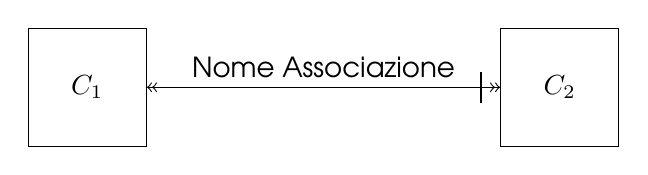
\begin{tikzpicture}[node distance=6cm, scale=2, main/.style={rectangle, draw, minimum size=15mm}]
        \node[main] (1) {$C_1$};
        \node[main] (2) [right of=1]{$C_2$};
        \draw[<<->>] (1) -- (2) node[midway, above] {Nome Associazione};
        \draw (2.5, 0.1) -- (2.5, -0.1);
    \end{tikzpicture}
    \caption{In questo caso abbiamo un'associazione \emph{multivalore} da entrambe la parti, ma \emph{parziale} per $C_2$ e \emph{totale} per $C_1$}
\end{figure}

\begin{figure}[h]
    \centering
    \captionsetup{justification=centering}
    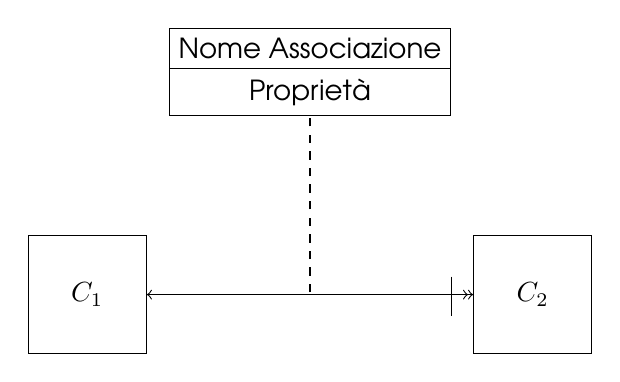
\begin{tikzpicture}[node distance=4cm, scale=2, main/.style={rectangle, draw, minimum size=15mm}]
        \node[rectangle split, rectangle split parts=2, draw] (prop) {Nome Associazione \nodepart{second} Proprietà};
        \node[main] (1) [below left of=prop]{$C_1$};
        \node[main] (2) [below right of=prop]{$C_2$};
        \draw[<->>] (1) -- (2);
        \draw (0.9, -1.3) -- (0.9, -1.55);
        \draw[dashed] (0, -1.4) -- (prop);
    \end{tikzpicture}
    \caption{Le associazioni possono presentare \textcolor{purple}{proprietà}}
\end{figure}

\begin{figure}[h]
    \centering
    \captionsetup{justification=centering}
    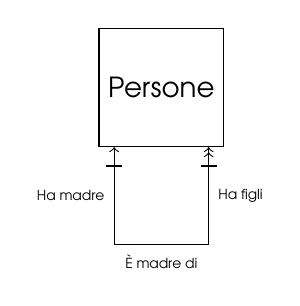
\begin{tikzpicture}[node distance=4cm, scale=2, main/.style={rectangle, draw, minimum size=15mm}]
        \node[main] (1) {Persone};
        \draw[->] (-0.3, -1) -- (-0.3, -0.38) node[midway, left] {\tiny{Ha madre}};
        \draw[->>] (0.3, -1) -- (0.3, -0.38) node[midway, right] {\tiny{Ha figli}};
        \draw[-] (-0.3, -1) -- (0.3, -1) node[midway, below] {\tiny{È madre di}};
        \draw[-] (-0.35, -0.5) -- (-0.25, -0.5);
        \draw[-] (0.25, -0.5) -- (0.35, -0.5);
    \end{tikzpicture}
    \caption{O possono anche essere \textcolor{purple}{ricorsive}. In questo caso occorre etichettare l'associazione non solo con il proprio nome, ma anche con i nomi dei ruoli che hanno le due entità nell'associazione.}
\end{figure}

\paragraph{\textcolor{purple}{Associazione Non Binarie}}
Le associazioni non binarie, per semplicità, non vengono rappresentate graficamente, ma ad esempio,
per quanto riguarda quelle \emph{ternarie}, queste vengono trasformate in tre associazioni \emph{binarie} aggiungendo un'altra
collezione al posto dell'associazione \emph{ternaria}.
    \subsection{Gerarchie}

Le classi di entità possono essere organizzate in una gerarchia di
\emph{specializzazione}. Una classe della gerarchia minore viene chiamata
\textbf{\textcolor{purple}{sottoclasse}}, mentre le altre si chiamano
\textbf{\textcolor{purple}{superclassi}}. Gli elementi di una sottoclasse
sono un sottoinsieme degli elementi della superclasse.

\subsubsection{Tipi Oggetto}

Fra i \emph{tipi oggetto} viene definita una relazione di sottotipo, che comprende le seguenti proprietà:
\begin{itemize}
    \item È una relazione \textcolor{purple}{asimmetrica}, \textcolor{purple}{riflessiva} e
        \textcolor{purple}{transitiva}.
    \item Inoltre, se un tipo $T$ è \emph{\textcolor{purple}{sottotipo}} di $T'$, allora
        tutti gli elementi di $T$ possono essere usati in tutti i contesti in cui appaiono elementi
        di tipo $T'$. Questa proprietà è chiamata \textcolor{purple}{sostitutività} ed è data dal fatto
        che gli elementi di $T$ hanno tutte le proprietà degli elementi di $T'$, e per ogni proprietà di $T'$,
        il suo tipo in $T$ è un sottotipo di quello che ha in $T'$. 
\end{itemize}

\paragraph{\textcolor{purple}{Ereditarietà}} L'\emph{ereditarietà} è una proprietà delle gerarchie
che permette di definire un \emph{tipo oggetto} a partire da un altro. In quanto, nel nostro contesto,
a partire da un tipo, si vuole solo definire un sottotipo, si parla di \emph{ereditarietà stretta}, che permette solo:
\begin{itemize}
    \item L'aggiunta di altri \emph{attributi}.
    \item La ridefinizione di attributi del \emph{supertipo}, però solo specializzando ulteriormente il tipo dell'attributo.
\end{itemize}

\subsubsection{Classi}

Fra le \emph{classi}, invece, viene definita una relazione di sottoclasse, con le seguenti proprietà:
\begin{itemize}
    \item Sempre \textcolor{purple}{asimmetrica}, \textcolor{purple}{riflessiva} e
        \textcolor{purple}{transitiva}, come per i \emph{tipi oggetto}.
    \item Se una classe $C$ è \emph{\textcolor{purple}{sottoclasse}} di $C'$, allora il tipo degli elementi di
        $C$ è sottotipo del tipo degli elementi di $C'$ (\textbf{\textcolor{purple}{vincolo intensionale}}).
    \item Se $C$ è \emph{\textcolor{purple}{sottoclasse}} di $C'$, allora gli elementi di $C$ sono un sottoinsieme
        degli elementi di $C'$ (\textbf{\textcolor{purple}{vincolo estensionale}}).
\end{itemize}

\paragraph{\textcolor{purple}{Vincoli}} Possiamo distinguere due tipi di vincoli su insiemi di sottoclassi:
\begin{itemize}
    \item \textcolor{purple}{Disgiunzione}: ogni coppia di sottoclassi nell'insieme è \emph{disgiunta}, quindi è priva di elementi comuni.
    \item \textcolor{purple}{Copertura}: l'unione degli elementi delle sottoclassi coincide con l'insieme degli elementi della \emph{superclasse}.
\end{itemize}

Se possiedono entrambi i vincoli, allora l'insieme delle \emph{sottoclassi} forma una \textcolor{purple}{partizione} della \emph{superclasse}. Altrimenti se nessuno
dei due vincoli è rispettato, si dice che le sottoclassi sono \textcolor{purple}{scorrelate}.

\begin{figure}[h]
    \centering
    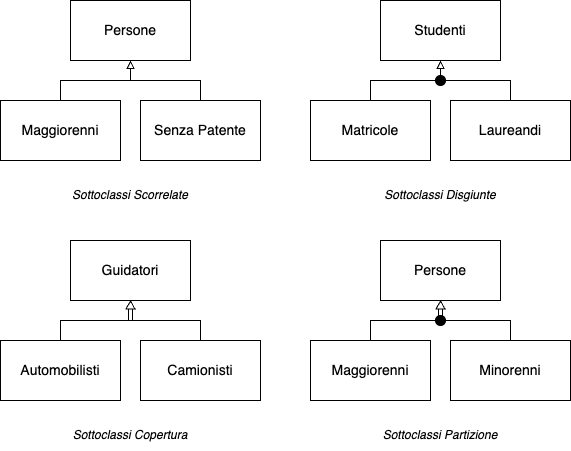
\includegraphics[scale=0.6]{img/gerarchie.png}
\end{figure}

\subsubsection{Ereditarietà Multipla}

Un tipo può anche essere definito per \emph{ereditarietà} anche a partire da più di un
\emph{supertipo}. Questo però può creare alcuni problemi quando lo stesso \emph{attributo} viene ereditato
da più di un supertipo, ma i tipi degli attributi fra loro sono diversi.
    \section{Progettazione Logica}

\subsection{Relazioni}

\begin{definition}[Relazione Matematica]
    Una \emph{relazione matematica} è un insieme di \emph{n}-uple ordinate
    $(d_1, \dots, d_n)$ tali che $d_1 \in D_1, \dots, d_n \in D_n$.

    Essendo un insieme, non c'è ordinamento fra le \emph{n}-uple, che inoltre devono essere
    tutte distinte. Però l'ordinamento all'interno della \emph{n}-upla conta, infatti l'\emph{i}-esimo
    valore deve provenire dall'\emph{i}-esimo dominio. Per questo si dice che la struttura della relazione
    è \emph{\textcolor{purple}{posizionale}}.
\end{definition}

\begin{definition}[Attributo]
    A ciascun dominio della relazione si associa un nome, chiamata \textbf{\textcolor{purple}{attributo}}.
\end{definition}

\begin{definition}[Tupla]
    Una \textbf{\textcolor{purple}{tupla}} su un insieme di \emph{attributi} chiamato $X$, è una funzione
    $t$ che associa a ciascun \emph{attributo} un valore del suo \emph{dominio}.

    Una \emph{\textcolor{purple}{relazione su $X$}} è un insieme di \emph{tuple}
    su $X$.
\end{definition}

\subsection{Tabelle}
Una \textbf{\textcolor{purple}{tabella}} rappresenta una relazione se:
\begin{itemize}
    \item I valori di ogni \emph{colonna} sono fra loro \emph{omogenei}.
    \item Le \emph{righe} sono tutte \emph{diverse} fra loro.
    \item Le \emph{intestazioni} delle colonne sono tutte \emph{diverse} fra loro.
\end{itemize}

In una \emph{tabella} l'ordinamento tra le righe e le colonne è irrilevante.

In ogni tabella è possibile distinguere due parti:
\begin{itemize}
    \item Lo \textbf{\textcolor{purple}{schema}} è rappresentato dalle intestazioni della tabella, che sono invarianti nel tempo e descrivono la
        struttura della tabella (\textbf{\textcolor{purple}{aspetto intensionale}}).
    \item L'\textbf{\textcolor{purple}{istanza}} sono i valori attuali presenti nella tabella, che
        possono cambiare nel tempo (\textbf{\textcolor{purple}{aspetto estensionale}}).
\end{itemize}

\begin{definition}[Tipo Ennupla]
    Un \textcolor{purple}{tipo ennupla} chiamato $T$ è un insieme finito di coppie (\emph{Attributo}, \emph{Tipo Elementare}).
\end{definition}

\begin{definition}[Schema di Relazione]
    Se $T$ è un \emph{tipo ennupla}, allora $R(T)$ è lo \textcolor{purple}{schema della relazione $R$}.
\end{definition}

\begin{definition}[Schema di Database]
    Lo \textcolor{purple}{schema di un database} è un insieme di \emph{schemi di relazioni} $R_i(T_i)$.
\end{definition}

\begin{definition}[Istanza di Relazione]
    Un'\textcolor{purple}{istanza di relazione}, anche chiamata \textbf{\textcolor{purple}{relazione}} su uno
    schema $R(T)$ è l'insieme $r$ di tuple di tipo $T$.
\end{definition}

\begin{definition}[Istanza di Database]
    Un'\textcolor{purple}{istanza di database} su uno schema $R=\{R_1(T_1), \dots, R_n(T_n)\}$
    è l'insieme delle \emph{relazioni} $r=\{r_1, \dots, r_n\}$, dove $r_i$ è un'\emph{istanza di relazione} su $R_i(T_i)$.
\end{definition}

\paragraph{Valore Nullo} Si indica con \verb|NULL|, e indica l'assenza di un valore del dominio.

\subsection{Vincoli di Integrità}
Un \textbf{\textcolor{purple}{vincolo d'integrità}} è una proprietà che deve
essere soddisfatta da ogni singola \emph{istanza} della relazione, in modo tale che rappresenti informazioni
corrette per l'applicazione.

Il vincolo viene espresso mediante un predicato, che associa ad ogni \emph{istanza} il valore \emph{\textcolor{Green}{vero}}
o \emph{\textcolor{red}{falso}}.

I vincoli si possono classificare in:
\begin{itemize}
    \item Vincoli \textcolor{purple}{intrarelazionali}: ovvero quelli che devono essere rispettati da valori della relazioni presa in considerazione, e possono essere:
        \begin{itemize}
            \item Vincoli sul \textcolor{purple}{dominio}, che coinvolgono un solo \emph{attributo}.
            \item Vincoli di \textcolor{purple}{ennupla}, che esprimono condizioni sui valori di ogni ennupla, indipendentemente dalle altre ennuple.
        \end{itemize}
    \item Vincoli \textcolor{purple}{interrelazionali}: sono quei vincoli che devono essere rispettati da valori presenti in relazioni diverse.
\end{itemize}

\subsection{Chiavi}

\begin{definition}[Superchiave]
    Un insieme $K$ di attributi viene chiamato \textbf{\textcolor{purple}{superchiave}} per una
    relazione $r$, se $r$ non contiene due ennuple distinte $t_1, t_2$ tali che $t_1[K] = t_2[K]$.
\end{definition}

\begin{definition}[Chiave]
    $K$ invece viene definito \textbf{\textcolor{purple}{chiave}} per $r$ se è una \emph{\textcolor{purple}{superchiave minimale}} per $r$, ovvero
    non deve contenere altre \emph{superchiavi}.
\end{definition}
    \subsection{Rappresentazione delle Associazioni}

\paragraph{\textcolor{purple}{Uno a Molti}}
Le associazioni \emph{uno a molti} si rappresentano aggiungendo, agli attributi
della relazione rispetto alla quale l'associazione è univoca, una
\emph{chiave esterna} che si riferisce all'altra relazione. Nel caso in
cui l'associazione ha degli attributi si aggiungono anch'essi alla relazione.

\begin{figure}[H]
    \centering
    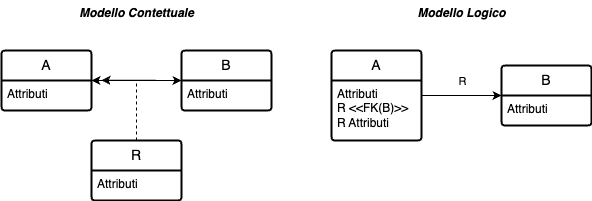
\includegraphics[scale=0.55]{img/unomolti.png}
\end{figure}

\paragraph{\textcolor{purple}{Uno a Uno}}
In questo caso si aggiunge la \emph{chiave esterna}
scegliendo arbitrariamente una delle due relazioni ma, in caso in
cui esiste un vincolo di totalità, si preferisce la relazione
rispetto alla quale l'associazione è \emph{totale}.

\begin{figure}[H]
    \centering
    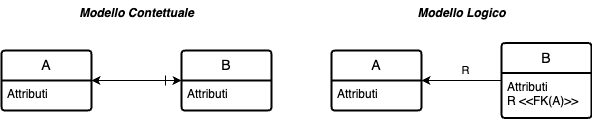
\includegraphics[scale=0.55]{img/unouno.png}
\end{figure}

\paragraph{\textcolor{purple}{Vincoli sulle Cardinalità}} La direzione dell'associazione
rappresentata dalla \emph{chiave esterna} è chiamata la \emph{\textcolor{purple}{diretta}}
dell'associazione. Per imporre un vincolo di \textcolor{purple}{univocità} della diretta occorre definire
un vincolo di chiave sulla \emph{chiave esterna}; mentre per descrivere un vincolo di \textcolor{purple}{totalità}
della diretta si impone un vincolo \verb|NOT NULL| sempre sulla \emph{chiave esterna}.

\paragraph{\textcolor{purple}{Molti a Molti}}
Un'associazione \emph{molti a molti} si traduce aggiungendo tra
le due relazioni, una terza che ha come attributi (e come \emph{chiave primaria})
le \emph{chiavi primarie} delle due relazioni.

\begin{figure}[H]
    \centering
    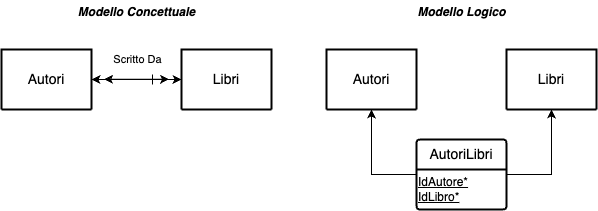
\includegraphics[scale=0.55]{img/moltimolti.png}
\end{figure}

\paragraph{\textcolor{purple}{Ricorsione}}
In questo caso la \emph{chiave esterna} si aggiunge alla stessa e sola
relazione.

\begin{figure}[H]
    \centering
    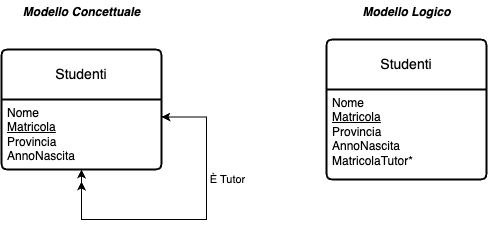
\includegraphics[scale=0.55]{img/ricorsioneunomolti.png}
\end{figure}

\paragraph{\textcolor{purple}{Ricorsione Molti a Molti}}
Anche qui si costruisce una seconda relazione che ha come \emph{chiave primaria}
le due \emph{chiavi primarie} delle due istanze coinvolte.

\begin{figure}[H]
    \centering
    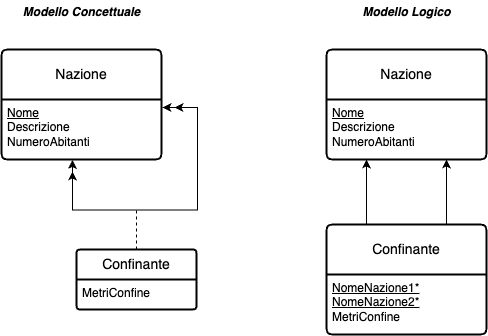
\includegraphics[scale=0.55]{img/ricorsionemoltimolti.png}
\end{figure}

\subsection{Rappresentazione delle Gerarchie}
Le \emph{gerarchie} non possono essere rappresentate direttamente, quindi
vanno eliminate sostituendole con altre classi e relazioni.

Ci sono tre metodi:
\begin{itemize}
    \item \textbf{\textcolor{purple}{Relazione Unica}}: se $A_0$ è la classe genitore di $A_1$ e $A_2$, queste vengono
        eliminate e accorpate ad $A_0$. Ad $A_0$ viene aggiunto un attributo chiamato \textcolor{purple}{discriminatore},
        che indica per ogni istanza da quale classe figlia deriva. Ovviamente anche gli attributi delle classi figlie
        vengono assorbite dal genitore e assumono valore \verb|NULL| sulle istanze di una classe figlia che non possedeva quegli
        attributi. Per quanto riguarda le relazioni, invece, anche queste vengono assorbite dalla classe genitore ma avranno
        comunque cardinalità minima uguale a 0, anche qui per le istanze di una classe figlia che non aveva quella relazione.
    \item \textbf{\textcolor{purple}{Partizionamento Orizzontale}}: la classe genitore $A_0$ viene eliminata e le classi figlie $A_1$
        e $A_2$ ereditano gli attributi e le relazioni del genitore. L'unico caso in cui non si può adoperare questo metodo è quando
        è presente un \emph{vincolo referenziale} verso la classe genitore, in quanto non è possibile spezzare il vincolo
        in più relazioni diverse.
    \item \textbf{\textcolor{purple}{Partizionamento Verticale}}: la gerarchia si trasforma in tante associazioni \emph{uno a uno}
        che legano ogni classe figlia con la classe genitore. In questo caso vanno aggiunti dei vincoli, ovvero ogni istanza di
        $A_0$ non può partecipare a tutte le associazioni, ma ad al più una; e nel caso in cui la gerarchia
        è totale deve essere esattamente 1.
        \paragraph{\textcolor{purple}{Nota Bene}} In quest'ultimo metodo la \emph{chiave primaria} della classe genitore
        è sia \emph{chiave esterna} che \emph{chiave primaria} per le figlie.
\end{itemize}

\subsection{Rappresentazione Campi Multivalore}
Per la gestione dei \emph{\textcolor{purple}{campi multivalore}} viene creata una nuova relazione
che ha come attributi il nome del campo e una \emph{chiave esterna} che si riferisce alla relazione in cui si
trovava. La \emph{chiave primaria} di questa nuova relazione è l'intera ennupla.
    \section{Algebra Relazionale}

\begin{definition}[Algebra Relazionale]
    Con \textbf{\textcolor{purple}{algebra relazionale}} si intende un
    insieme di \emph{operatori} su relazioni che danno come risultato altre relazioni.
    Non viene usato come linguaggio di interrogazione dei \emph{DBMS}, ma come rappresentazione
    interna delle interrogazioni.
\end{definition}

\subsection{Operatori Insiemistici}
Le relazioni vengono viste come degli \emph{\textcolor{purple}{insiemi}}.
Gli operatori di \emph{\textcolor{purple}{unione}}, \emph{\textcolor{purple}{differenza}}
ed \emph{\textcolor{purple}{intersezione}} sono applicabili solo a relazioni
definite sugli stessi \emph{attributi}.
\begin{itemize}
    \item \textbf{\textcolor{purple}{Unione}}: l'unione di due relazioni $R$ e $S$ definite
        sullo stesso insieme di attributi $X$ è indicata con $R \cup S$ ed è una relazione su $X$
        che contiene le tuple che appartengono a $R$ o a $S$ senza ripetizioni.
    \item \textbf{\textcolor{purple}{Differenza}}: la differenza è indicata con $R - S$ ed è una relazione sempre su
        $X$ che contiene tutte le tuple che appartengono ad $R$ ma non a $S$.
    \item \textbf{\textcolor{purple}{Ridenominazione}}: è un operatore \emph{\textcolor{purple}{monadico}}, ovvero su una sola relazione, che permette
        di modificare lo schema, ridenominando il nome di uno o più attributi, ma lasciando inalterate le istanze.
        \begin{center}
            $\rho_{\;Nuovo\;Nome\;Attributo\;\leftarrow\;Vecchio\;Nome\;Attributo}\;(Relazione)$
        \end{center}
    \item \textbf{\textcolor{purple}{Proiezione}}: è un altro operatore \emph{monadico} che produce un
        risultato su un sottoinsieme degli attributi della relazione e contiene le ennuple della
        relazione ristrette solo agli attributi del sottoinsieme.
        \begin{center}
            $\pi_{\;Lista\;Attributi}\;(Relazione)$
        \end{center}
        La cardinalità di una \emph{proiezione} è basata sul sottoinsieme $X$ degli
        attributi:
        \begin{itemize}
            \item Se $X$ è una \emph{superchiave} di $R$, allora $\pi_{X}(R)$ contiene esattamente
                tante ennuple quante ne contiene $R$.
            \item Altrimenti se $X$ non è \emph{superchiave}, potrebbero essere presenti dei valori che
                su quegli attributi sono ripetuti e che quindi vengono rappresentati una sola volta.
        \end{itemize}
    \item \textbf{\textcolor{purple}{Selezione}} o \textbf{\textcolor{purple}{Restrizione}}: è sempre un operatore
        \emph{monadico} che produce una relazione con lo stesso schema dell'operando, che contiene un sottoinsieme delle sue ennuple
        che soddisfano una data condizione.
        \begin{center}
            $\sigma_{\;Cond}\;(R)$
        \end{center}
        Con $Cond$ generata dalla seguente grammatica: \\ \\
        \verb+ Cond ::= Exp Theta Exp | Cond And Cond | Cond Or Cond | Not Cond + \\
        \verb+ Exp ::= Attributo | Costante | Exp Op Exp + \\
        \verb+ Theta ::= = | < | > | != | <= | >=+ \\
        \verb1 Op ::= + | - | * | StringConcat 1 \\ \\
        Le condizioni atomiche si riferiscono solo ai valori non nulli, per riferirsi anche
        ai valori nulli si usano forme di condizioni come \verb|IS NULL| e \verb|IS NOT NULL|.
    \item \textbf{\textcolor{purple}{Prodotto}}: operatore fra più relazioni che devono avere
        fra loro tutti i nomi degli attributi distinti, e che esegue il prodotto cartesiano fra gli
        insiemi di tuple.
    \item \textbf{\textcolor{purple}{Intersezione}}: l'intersezione è indicata con $R \cap S$ ed è una relazione definita
        sullo stesso insieme di attributi $X$ che contiene le tuple che appartengono sia ad $R$ che ad $S$.
        L'\emph{intersezione} è chiamato operatore \emph{\textcolor{purple}{derivato}}, dato che è possibile derivarlo usando altri
        operatori:
        \begin{center}
            $R \cap S \; = \; \{x \;|\; x \in R \land \exists \; y \in S \;t.c.\; x = y \}$
        \end{center}
        allora se per esempio $R$ ed $S$ sono definiti con $X = \{A, B\}$.
        \begin{center}
            $\pi_{A, B}(\sigma_{A=S.A\;AND\;B=S.B}(R \times \rho_{S}(S)))$
        \end{center}
        Partendo dall'interno, si ridenominano tutti gli attributi di $S$ ponendogli davanti
        il prefisso $S$, successivamente viene fatto il \emph{prodotto} con $R$ e tramite la
        \emph{selezione} selezioniamo solo le tuple che hanno gli attributi semanticamente uguali con
        gli stessi valori. Infine si fà una \emph{proiezione} per eliminare gli attributi ridondanti.
\end{itemize}

\subsubsection{Join}
Il \textbf{\textcolor{purple}{join}} o \textbf{\textcolor{purple}{giunzione}} permette di
correlare dati in relazioni diverse. Anch'esso è un operatore derivato in quanto si può ottenere per composizione
degli operatori visti precedentemente. Si indica con il simbolo $\bowtie$.

Il \textbf{\textcolor{purple}{join naturale}} produce un'unione degli attributi dei due operandi, combinando le ennuple
degli operandi che hanno valori uguali sugli attributi in comune. Ad esempio $R_1 \bowtie R_2$ è una relazione su $X_1 \cup X_2$ definita come segue:
\begin{center}
    $R_1 \bowtie R_2 = \{t \;su\; X_1 \cup X_2 \;|\; esistono \;t_1 \in R_1 \;e\; t_2 \in R_2 $ \\
    $\;con\; t[X_1] = t_1 \;e\; t[X_2] = t_2\}$
\end{center}

Un \emph{join} viene chiamato \emph{\textcolor{purple}{completo}} se ogni ennupla delle due relazioni
contribuisce al risultato. Al contrario si parla di \emph{join} \emph{\textcolor{purple}{non completo}}.
Generalmente possiamo definire un limite inferiore e superiore alla cardinalità di una join:
\begin{center}
    $0 \leq |R_1 \bowtie R_2| \leq |R_1| \times |R_2|$
\end{center}
Nel caso il join è \emph{completo} possiamo restringere il limite inferiore
dicendo che $|R_1 \bowtie R_2| \geq \max\{|R_1|, |R_2|\}$.
\\\\
Nel caso in cui il join coinvolge come attributo comune una \emph{chiave} di $R_2$, allora:
\begin{center}
    $0 \leq |R_1 \bowtie R_2| \leq |R_1|$
\end{center}

Se oltre a coinvolgere una \emph{chiave} di $R_2$, vi è un vincolo di \emph{integrità referenziale} tra un
attributo di $R_1$ e la chiave di $R_2$ allora la cardinalità della join è esattamente $|R_1|$.
\\\\
Un \textbf{\textcolor{purple}{join esterno}} estende con valori nulli le ennuple che verrebbero
tagliate fuori da un \emph{\textcolor{purple}{join naturale}}.
Esiste in tre versioni:
\begin{itemize}
    \item \textcolor{purple}{Join esterno sinistro} $R \overset{\leftarrow}{\bowtie} S$: mantiene tutte le ennuple del primo
        operando, estendendole con valori nulli se necessario.
    \item \textcolor{purple}{Join esterno destro} $R \overset{\rightarrow}{\bowtie} S$: mantiene tutte le ennuple del secondo
    operando, estendendole con valori nulli se necessario.
    \item \textcolor{purple}{Join esterno completo} $R \overset{\leftrightarrow}{\bowtie} S$: mantiene tutte le ennuple di entrambi
        gli operandi, estendendole con valori nulli se necessario.
\end{itemize}

\paragraph{\textcolor{purple}{Nota Bene}} Il \emph{prodotto cartesiano} si può
vedere come un \emph{join naturale} su relazioni che non hanno attributi in comune.
\\ \\
Dato che il \emph{\textcolor{purple}{prodotto cartesiano}} non ha senso se non
lo facciamo seguire da una selezione (che permette di specificare la condizione sui campi
che semanticamente rappresentano lo stesso attributo), si usa l'operazione di
\textbf{\textcolor{purple}{theta-join}} definito come segue:
\begin{center}
    $R_1 \bowtie_{\;Condizione} R_2$
\end{center}
che è equivalente a:
\begin{center}
    $\sigma_{\;Condizione}\;(R_1 \bowtie R_2)$
\end{center}
\textbf{N.B.}: dato che $R_1$ ed $R_2$ non hanno attributi comuni, in
questo caso $\bowtie \;= \times$.

Se nel \emph{theta-join} l'operatore di confronto nella $Condizione$ è sempre
l'uguaglianza, allora si parla di \textbf{\textcolor{purple}{equi-join}}.

\paragraph{\textcolor{purple}{Self Join}} Supponiamo di avere questa relazione \verb|Genitori|:
\begin{center}
    \begin{tabular}{|c|c|}
        \hline
        \rowcolor{purple}
        \textcolor{white}{Genitore} & \textcolor{white}{Figlio} \\
        \hline
        Luca & Anna \\
        \hline
        Maria & Anna \\
        \hline
        Giorgio & Luca \\
        \hline
        Silvia & Maria \\
        \hline
        Enzo & Maria \\
        \hline
    \end{tabular}
\end{center}

e di voler ottenere una relazione \verb|Nonno-Nipoti|. Per far ciò occorre riutilizzare la stessa
tabella ma facendo $Genitori \bowtie Genitori$ si otterrebbe di nuovo la tabella \verb|Genitori|.
In questo caso occorre ridenominare la tabella due volte:

\begin{table}[H]
    \parbox{.55\linewidth}{
    \centering
    \begin{tabular}{|c|c|}
        \hline
        \rowcolor{purple}
        \textcolor{white}{Nonno} & \textcolor{white}{Genitore} \\
        \hline
        Luca & Anna \\
        \hline
        Maria & Anna \\
        \hline
        Giorgio & \textcolor{blue}{Luca} \\
        \hline
        Silvia & \textcolor{red}{Maria} \\
        \hline
        Enzo & \textcolor{red}{Maria} \\
        \hline
    \end{tabular}
    \caption{$\rho_{\;Nonno,\;Genitore \leftarrow Genitore,\;Figlio}(Genitore)$}
    }
    \hfill
    \parbox{.45\linewidth}{
    \centering
    \begin{tabular}{|c|c|}
        \hline
        \rowcolor{purple}
        \textcolor{white}{Genitore} & \textcolor{white}{Nipote} \\
        \hline
        \textcolor{blue}{Luca} & Anna \\
        \hline
        \textcolor{red}{Maria} & Anna \\
        \hline
        Giorgio & Luca \\
        \hline
        Silvia & Maria \\
        \hline
        Enzo & Maria \\
        \hline
    \end{tabular}
    \caption{$\rho_{\;Nipote \leftarrow Figlio}(Genitore)$}
    }
\end{table}
Infine, effettuando una \emph{join} seguita da una \emph{proiezione} otteniamo:
\begin{center}
    \begin{tabular}{|c|c|}
        \hline
        \rowcolor{purple}
        \textcolor{white}{Nonno} & \textcolor{white}{Nipote} \\
        \hline
        Giorgio & Anna \\
        \hline
        Silvia & Anna \\
        \hline
        Enzo & Anna \\
        \hline
    \end{tabular}
\end{center}

\begin{center}
    $\pi_{\;Nonno,\;Nipote}(\rho_{\;Nonno,\;Genitore \leftarrow Genitore,\;Figlio}(Genitore) \bowtie \rho_{\;Nipote \leftarrow Figlio}(Genitore))$
\end{center}

    \end{sloppypar}
\end{document}